% !TeX spellcheck = es_ES
\documentclass[12pt, titlepage]{article}
\usepackage[utf8]{inputenc}
\usepackage[spanish]{babel}
\usepackage{float}
\usepackage[letterpaper, margin=2.5cm]{geometry}
\usepackage[nottoc,notlot,notlof]{tocbibind} % Hace que se agregen las referencias al indice
\usepackage{url}
\usepackage{graphicx} 
\usepackage{listings}
\usepackage{color}
\definecolor{dkgreen}{rgb}{0,0.6,0}
\definecolor{gray}{rgb}{0.5,0.5,0.5}
\definecolor{mauve}{RGB}{253,151,31}

\lstset{frame=tb,
    language=Sql,
    aboveskip=3mm,
    belowskip=3mm,
    showstringspaces=false,
    columns=flexible,
    basicstyle={\small\ttfamily},
    numbers=none,
    numberstyle=\tiny\color{gray},
    keywordstyle=\color{blue},
    commentstyle=\color{dkgreen},
    stringstyle=\color{mauve},
    breaklines=true,
    breakatwhitespace=true,
    tabsize=2,
    morekeywords={use}
}

\title{Practica 2}
\author{Carlos Tonatihu Barrera Pérez \\ Profesor: Hernández Contreras Euler \\ Bases de Datos \\ Grupo: 2CM1 }
\date{27 de febrero de 2017}

\begin{document}
    \maketitle
    \tableofcontents
    \section{Marco Teórico}
    hola
    \section{Desarrollo}
        El primer paso en esta practica fue crear la base de datos que se iba a utilizar junto a las relaciones que la integrarían, para esto se utilizaron los siguientes comandos.
        \begin{lstlisting}
            create database cine; --Crea la base de datos
            use cine; -- Necesario para poder trabajar con la base recien creada
        \end{lstlisting}
        \begin{figure}[H]
            \begin{center}
                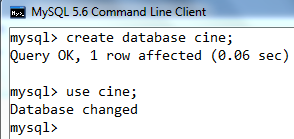
\includegraphics[width=12cm, height=6cm]{img/hasta-use.png}
                \caption{Creación y uso de la base.}
                \label{fig:hasta-use}
            \end{center}
        \end{figure}
    Se crean las tablas empleado, cinemex y ec.
        \begin{lstlisting}
        create table empleado(
            idEmp int not null primary key,
            nombre varchar(30),
            dir varchar(100),
            tel int,
            genero varchar(10)
        );
        
        create table cinemex(
            idCinemex int not null primary key,
            nombre varchar(50),
            dir varchar(100),
            tel int,
            email varchar(60)
        );
        
        create table ec(
            idEmp int not null,
            idCinemex int not null,
            primary key(idEmp, idCinemex),
            foreign key(idEmp) references empleado(idEmp) on delete cascade on update cascade,
            foreign key(idCinemex) references cinemex(idCinemex) on delete cascade on update cascade
        );
        \end{lstlisting}
        \begin{figure}[H]
            \begin{center}
                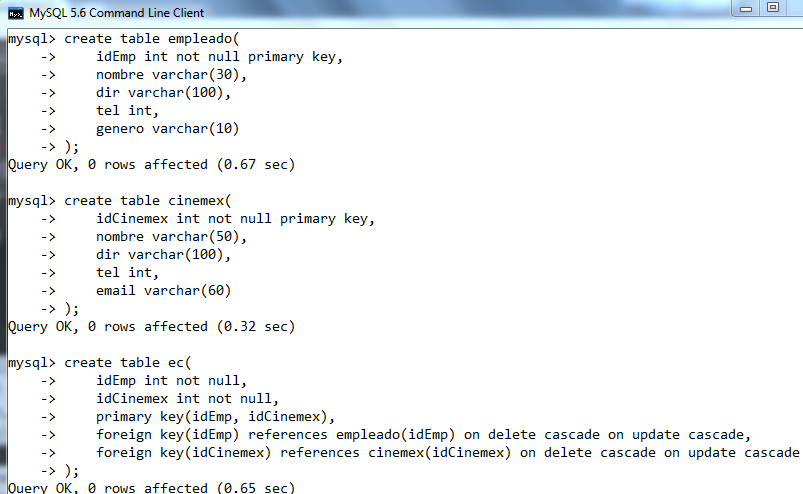
\includegraphics[width=16cm, height=10cm]{img/tablas.png}
                \caption{Creación de tablas.}
                \label{fig:tablas}
            \end{center}
        \end{figure}
    \begin{figure}[H]
        \begin{center}
            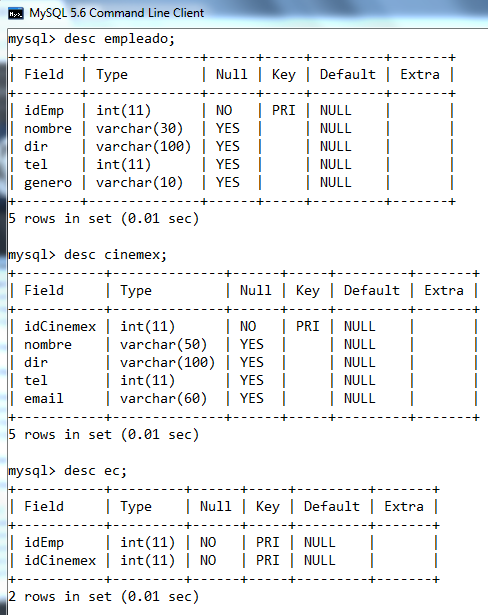
\includegraphics[width=12cm, height=10cm]{img/tablas-desc.png}
            \caption{Descripción.}
            \label{fig:desc}
        \end{center}
    \end{figure}
    Ahora comenzamos con la modificación de las tablas, primero agregamos 2 columnas que permitan almacenar el salario y el correo electrónico en los empleados.
    \begin{lstlisting}
    alter table empleado add column email varchar(60);
    alter table empleado add column salario double;
    \end{lstlisting}
    \begin{figure}[H]
        \begin{center}
            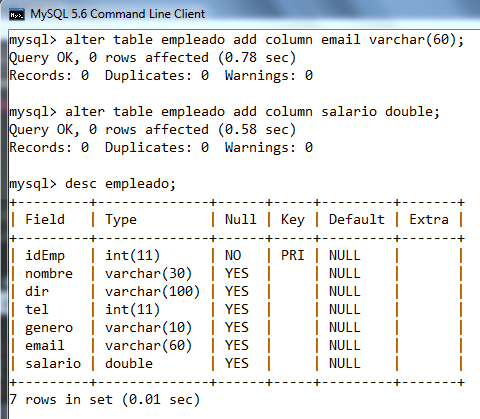
\includegraphics[width=10cm, height=11cm]{img/alter-table.png}
            \caption{Resultado del alter table.}
            \label{fig:arlter}
        \end{center}
    \end{figure}
    Después procedemos a crear una nueva relación gerente
     \begin{lstlisting}
    create table gerente(
        idGerente int not null primary key,
        nombre varchar(30),
        turno varchar(15),
        noCel int,
        salario double,
        idCinemex int,
        foreign key(idCinemex) references cinemex(idCinemex) on delete cascade on update cascade;
    );
    \end{lstlisting}
    \begin{figure}[H]
        \begin{center}
            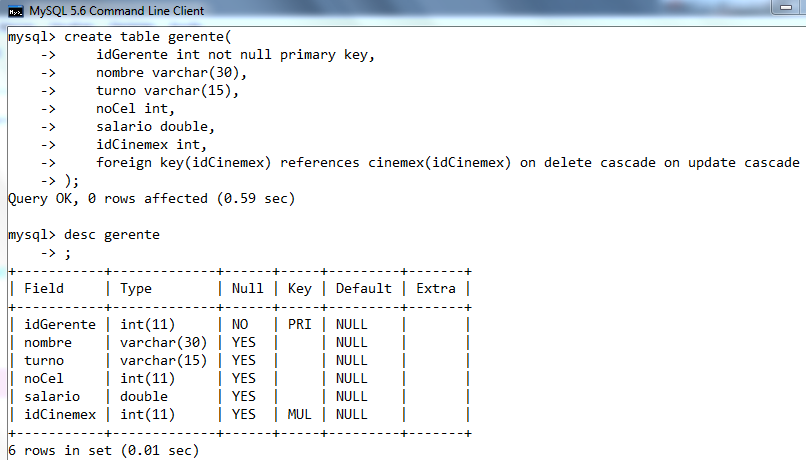
\includegraphics[width=14cm, height=10cm]{img/tabla-gerente.png}
            \caption{Nuestra nueva tabla.}
            \label{fig:tabla-gerente}
        \end{center}
    \end{figure}
    Ahora modificamos las gerente, empleado y asociado y observamos los cambios.
    \begin{lstlisting}
    -- Cambiar el tipo de dato del nocel del gerente a varchar
    alter table gerente modify column noCel varchar(15); --modifica la descripcion del tipo de dato
    
    -- Renombrar la relacion empleado a asociado
    alter table empleado rename as asociado; -- SOLO modifica el nombre
    
    -- Aumentar el tamano del tipo de dato de la dir en asociado
    alter table asociado modify column dir varchar(200); 
    \end{lstlisting}
    \begin{figure}[H]
        \begin{center}
            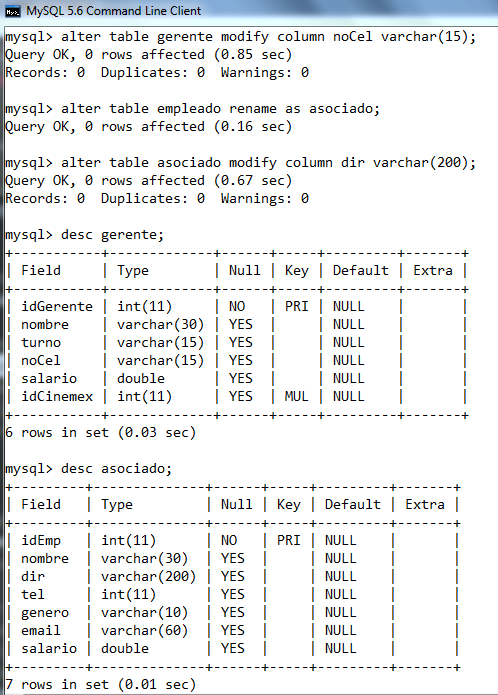
\includegraphics[width=10cm, height=10cm]{img/mas-alter.png}
            \caption{Los cambios que sucedieron.}
            \label{fig:alter2}
        \end{center}
    \end{figure}
    Procedemos a modificar la llave primaria de cinemex que ahora sera compuesta por el id y el nombre por lo que también se tienen que modificar las tablas que esten relacionadas con esta por lo que seguiremos los siguientes pasos:
    \begin{enumerate}  
        \item Eliminar PK de cinemex, pero antes eliminar la llave foranea con gerente y ec. 
        \item Definir PK compuesta.
    \end{enumerate}
    \begin{lstlisting}
    show create table gerente; -- Muestra la descripcionde la relacion de una forma mas completa a comparacion del comando desc para poder obtener el constraint de lo contrario no se podria eliminar la primary key de cinemex ya que es utilizada en esta relacion
    alter table gerente drop foreign key gerente_ibfk_1;
    \end{lstlisting}
    \begin{figure}[H]
        \begin{center}
            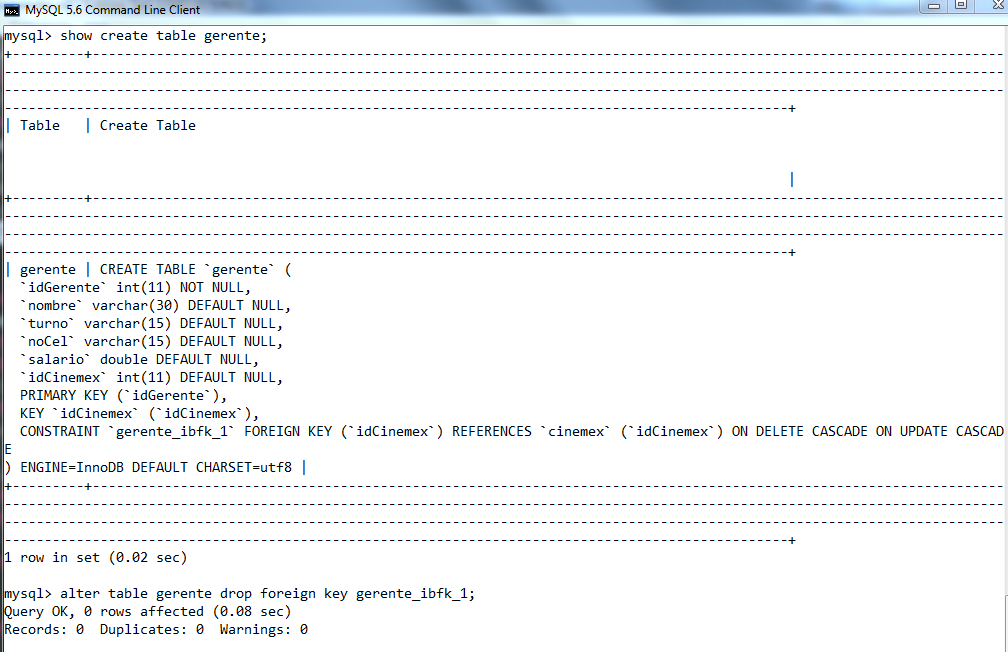
\includegraphics[width=15cm, height=11cm]{img/drop-fk.png}
            \caption{Los cambios que sucedieron.}
            \label{fig:drop-fk}
        \end{center}
    \end{figure}
    Lo mismo para ec pero hay que tener cuidado de no borrar la de la relación asociado. 
    \begin{lstlisting}
    show create table ec;
    alter table ec drop foreign key ec_ibfk_2;
    \end{lstlisting}
    \begin{figure}[H]
        \begin{center}
            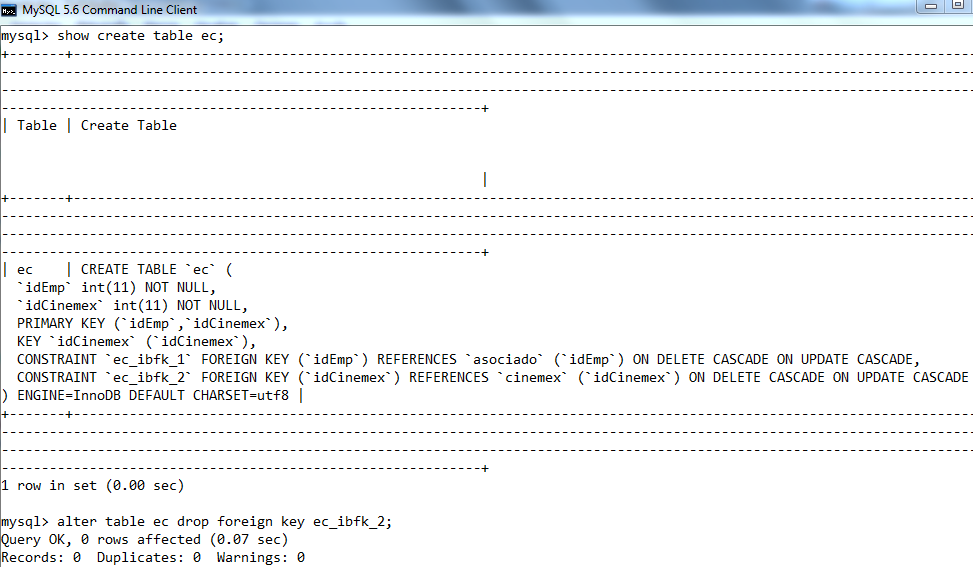
\includegraphics[width=15cm, height=11cm]{img/drop-fk2.png}
            \caption{Los cambios que sucedieron.}
            \label{fig:drop-fk2}
        \end{center}
    \end{figure}
    \begin{lstlisting}
    alter table cinemex drop primary key; -- Ahora si podemos eliminar la clave primaria
    alter table cinemex add primary key(idCinemex, nombre); -- Creamos nuestra nueva PK compuesta
    \end{lstlisting}
    \begin{figure}[H]
        \begin{center}
            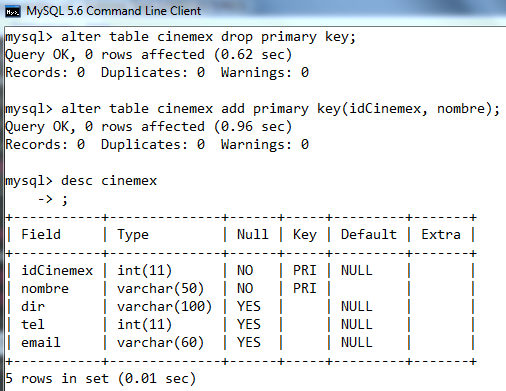
\includegraphics[width=10cm, height=10cm]{img/compuesta.png}
            \caption{Cambios en la tabla.}
            \label{fig:tabla}
        \end{center}
    \end{figure}
    Es necesario agregar el campo que falta para la relación y poder crear la clave foranea compuesta en las tablas de gerente y ec. Es importante que sean iguales al campo de la tabla cinemex aunque pueden llevar nombres distintos.
     \begin{lstlisting}
    alter table gerente add column nomCine varchar(50);
    alter table ec add column nomCine varchar(50);
    -- Se crea la FK compuesta
    alter table gerente add foreign key(idCinemex, nomCine) references cinemex(idCinemex, nombre) on delete cascade on update cascade;
    
    alter table ec add foreign key(idCinemex, nomCine) references cinemex(idCinemex, nombre) on delete cascade on update cascade;
    \end{lstlisting}
    \begin{figure}[H]
        \begin{center}
            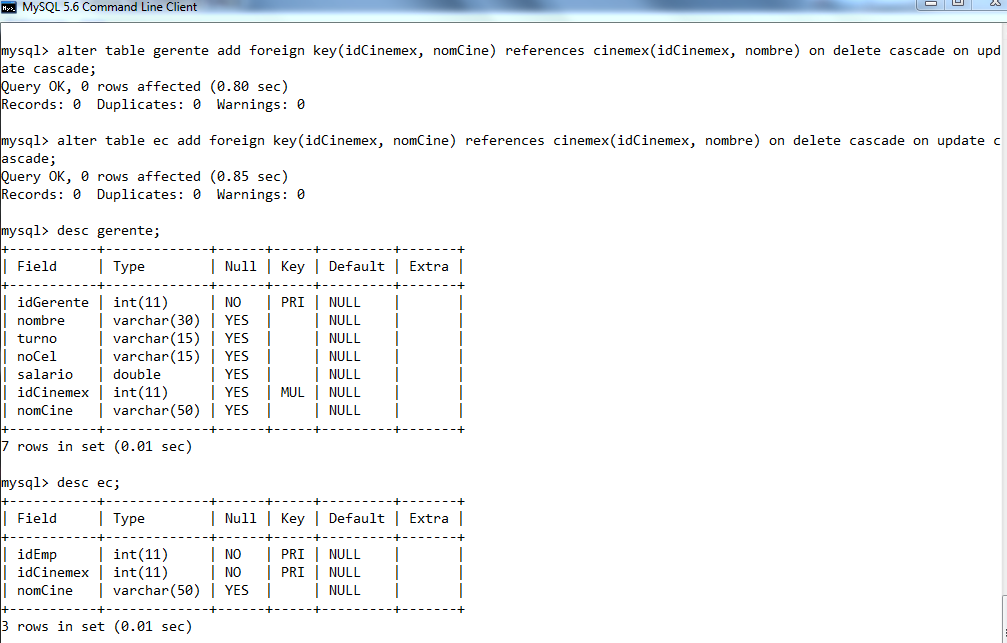
\includegraphics[width=16cm, height=11cm]{img/casi.png}
            \caption{Tablas modificadas.}
            \label{fig:modificaciones}
        \end{center}
    \end{figure}
    Por ultimo se crea la relación cartelera y se asocia con cinemex.
    \begin{lstlisting}
    create table cartelera(
        idCartelera int not null primary key,
        nombre varchar(50),
        fechaInicio date,
        fechaFin date,
        clasificacion varchar(5)
    );
    \end{lstlisting}
    \begin{figure}[H]
        \begin{center}
            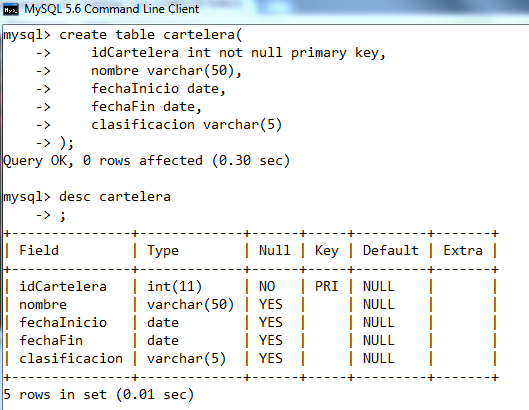
\includegraphics[width=16cm, height=11cm]{img/cartelera.png}
            \caption{Tablas modificadas.}
            \label{fig:foranea}
        \end{center}
    \end{figure}
    Finalmente creamos una llave foranea en cinemex que se asocia con la cartelera.
    \begin{lstlisting}
    alter table cinemex add column idCartelera int;
    alter table cinemex add foreign key(idCartelera) references cartelera(idCartelera) on delete cascade on update cascade;
    \end{lstlisting}
    \begin{figure}[H]
        \begin{center}
            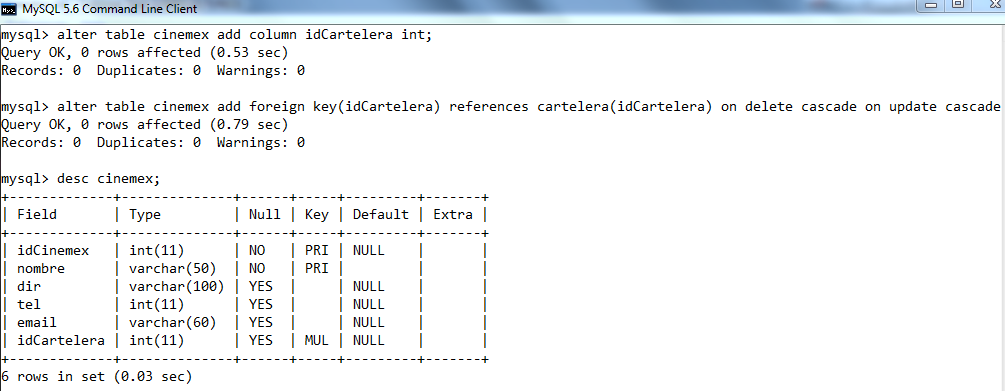
\includegraphics[width=16cm, height=10cm]{img/foranea-cartelera.png}
            \caption{Tablas modificadas.}
            \label{fig:foranea-cartelera}
        \end{center}
    \end{figure}
    Para terminar se exporto la base de datos a un archivo .sql
    \begin{figure}[H]
        \begin{center}
            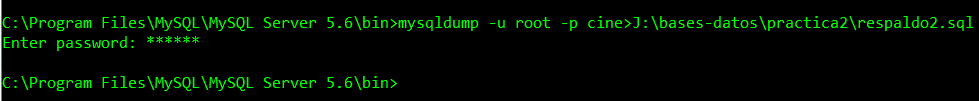
\includegraphics[width=16cm, height=3cm]{img/exportacion.png}
            \caption{Exportar la base.}
            \label{fig:exportacion}
        \end{center}
    \end{figure}
    \section{Conclusiones}
        Esta segunda práctica me permitió profundizar y reforzar lo aprendido en la primera práctica para poder aprender más rápida y clara los comandos que se usan en la creación y trabajo de una base de datos, a pesar de ser comandos básicos considero que pueden llegar a complicarse a medida de que la complejidad de una base de datos aumenta. Por lo que es importante continuar practicando para no olvidar el como se declara cada sentencia sql y no depender de guías salvo para casos mas complejos.
    \bibliography{bibliografia} 
    \bibliographystyle{ieeetr}
\end{document}